\chapter{Experiments}
\label{chap:experiments}

\minitoc \mtcskip \noindent

Providing to the final users of our framework actionable and trustful information about the smart cities and transportation domains is a laborious and time consuming process. First, in order to extract information it is necessary the conduction of some experiments to test the text analytics modules described in Section~\ref{sec:text_analytics}. Second, the results obtained from each experiment need to be evaluated in order to prove robustness and efficiency in our implemented modules. Last but not least, it is necessary to enhance the value and importance of such analysis and what indeed social media content can provide to improve services and the whole cities that use our framework.

Hence, in this Chapter, we describe three different experiments that were perform during this dissertation period to implement the previous mentioned text analytics modules

\section{Topic Modelling}\label{sec:topic_modeling}
This section is related to the experiment of automatically characterize tweets in two different Brazilian cities, Rio de Janeiro and São Paulo. We used an unsupervised learning approach to tackle the task of topic modelling in order to compare both cities and see if there are differences between topics people talked about. Automatic characterization of text messages is a laborious and time consuming task since it is necessary to assure the right level of abstraction in the learning model; very much similarly to human minds, which essentially present a bounded rationality nature, our learning model needs to be trained in order to assimilate the necessary knowledge and perform the appropriate analogies so as to discover different topics within the tweets' contents.

Messages collected to conduct this experiment are correspondent to a period of two months, between days March 12 and May 12, 2017. The resulting datasets sum up a total of 12.5M and 6.3M tweets for Rio de Janeiro and for São Paulo, respectively. Due to the problem detected in Section~\ref{sec:data_collection}, we filtered the data in order to only use the tweets that were actually inside the cities' areas. The final composition of the non-filtered datasets is presented in Table~\ref{tab:datasets}, and by observing its content it is possible to verify that almost 6M tweets were not located inside the cities' bounding-boxes.

\begin{table*}[ht]
	\small
	\centering
	\caption{Datasets composition}
	\label{tab:datasets}
	\resizebox{\textwidth}{!}{\begin{tabular}{|c|c|c|c|c|c|c|}
			\hline
			\textbf{City}  & \textbf{All} & \textbf{PT} & \textbf{Non-PT} & \textbf{\begin{tabular}[c]{@{}c@{}}In \\ Bounding-Box\end{tabular}} & \textbf{\begin{tabular}[c]{@{}c@{}}Out\\ Bounding-Box\end{tabular}} & \textbf{\begin{tabular}[c]{@{}c@{}}PT and \\ In Bounding-Box\end{tabular}} \\ \hline
			Rio de Janeiro & 12,531,000 & 10,570,000 & 1,961,000 & 8,644,000 & 3,886,000 & 7,353,000 \\ \hline
			São Paulo & 6,352,000 & 4,886,000 & 1,466,000 & 4,247,000 & 2,105,000 & 3,313,000 \\ \hline
		\end{tabular}}
	\end{table*}
	
After the filtering process, we select the subset of data composed by Portuguese tweets and located inside the cities' bounding-boxes, and used it to conduct the experiment described in this section. Such subset can be sum up to a total of 7.3M and 3.3M for Rio de Janeiro and São Paulo, respectively.

%Features and pre-processing operations are the ones described in Section~\ref{sec:topic_modelling}.

Usually, to tackle topic modelling tasks in text documents several pre-processing operations are needed in order to make its content as clean and correct as possible since, as previous mentioned in Section~\ref{sec:topic_modelling}, models responsible for this task handle with the most basic element in texts - words. The pre-processing of tweets increase the performance of the LDA model and removing unnecessary words, transforming words into their root form as so deleting all the punctuation are some of the common text mining pre-processing steps usually used in this type of analysis. Here, each tweet of both datasets was submitted to a specific and planned group of pre-processing operations, which are described in Section~\ref{sec:text_preprocessing}, and were used to train a LDA model and proceed with the experiment.
	
It is worth noting that, after the data preparation phase, 772,017 tweets have their message empty which means that its content is irrelevant for the final experiment phase.

\subsection{LDA Model Parametrization}
In order to understand and see the LDA model performance, we set five different numbers for the topics results parameter of the training process: 5, 10, 20, 25 and 50 topics, being this the one with better results. The number of iterations to train the model was set to 20, since our desire was to reproduce the experiment made by G. Lansley et al.~\cite{lansley2016geography}, which revealed interesting results regarding the characterization of land-uses in the city of London. Finally but not the least, each tweet in the datasets was treated as a single document comprehending that, in total, 6,580,983 different documents were used in the model training process.
	
\subsection{Results and Analysis}
\label{subsec:topic_modelling_results}
\label{subsec:lda_results}
To evaluate the experimental results obtained for each model (where the difference underlies on the variation of the number of topics), a list with the most frequent 50 words for each topic was extracted. In Table~\ref{tab:topics_classification} we can observe a sample (20 top words) selected out of the 50 studied. Nonetheless, the final evaluation took into consideration all the  50 outputted words.

\begin{table}[h]
	\centering
	\caption{Example of the topics classification}
	\label{tab:topics_classification}
	\resizebox{\textwidth}{!}{
		\begin{tabular}{c|c}
			\hline
			\textbf{\begin{tabular}[c]{@{}c@{}}Words\\ (only 20 words)\end{tabular}} & \textbf{\begin{tabular}[c]{@{}c@{}}Topic\\ Classification\end{tabular}} \\ \hline
			\begin{tabular}[c]{@{}c@{}}paulo, vai, hoje, dia, jogo, ser, melhor, time, vamo, brazil, \\ todo, santo, brasil, gol, cara, aqui, agora, corinthiam, ano, palmeiro, vem, ...\end{tabular} & \begin{tabular}[c]{@{}c@{}}Sports and\\ Games\end{tabular} \\ \hline
			\begin{tabular}[c]{@{}c@{}}vou, dia, dormir, queria, hoje, ficar, casa, semano, quero, ter, \\ ainda, hora, agora, sono, aula, acordar, acordei, cedo, fazer, prova, ...\end{tabular} & \begin{tabular}[c]{@{}c@{}}Wake-up\\ Messages\end{tabular} \\ \hline
			\begin{tabular}[c]{@{}c@{}}top, social, artist, vote, the, award, army, bom, voting, doi, \\ bogo, oitenta, sipda, today, vinte, prepara, cypher, oito, quatro, man, ...\end{tabular} & \begin{tabular}[c]{@{}c@{}}Voting and\\ Numbers\end{tabular} \\ \hline
			\begin{tabular}[c]{@{}c@{}}marco, nada, falar, emilly, gente, quer, nao, pessoa, nunca, fala, \\ vai, falando, sobre, chama, agora, manda, vem, mensagem, vivian, bbb, ...\end{tabular} & \begin{tabular}[c]{@{}c@{}}Big Brother\\ Brazil 2017\end{tabular} \\ \hline
			\begin{tabular}[c]{@{}c@{}}paulo, brazil, sao, santo, vila, just, parque, posted, photo, shopping, \\ paulista, centro, bernardo, jardim, cidade, avenido, praia, santa, campo, academia\end{tabular} & \begin{tabular}[c]{@{}c@{}}Tourism and\\ Places\end{tabular} \\ \hline
		\end{tabular}
	}
\end{table}
	
We also selected and manually analyse a random sample (with the size of 200) of tweets for each topic. This sampling was done in order to get better consistency and trustiness about the classification and characterization of the tweets.

\begin{table}[!hb]
	\centering
	\caption{Final results of the LDA topics aggregation}
	\label{tab:final_classification}
	\resizebox{\textwidth}{!}{
		\begin{tabular}{l|S[table-format=7.0]S[table-format=2.2]|S[table-format=7.0]S[table-format=2.2]|rS[table-format=2.2]}
			\hline
			\multicolumn{1}{c|}{\multirow{2}{*}{\textbf{Topic Group}}} & \multicolumn{2}{c|}{\textbf{Rio de Janeiro}} & \multicolumn{2}{c|}{\textbf{S\~ao Paulo}} & \multicolumn{1}{c}{\multirow{2}{*}{\textbf{Diff (\%)}}} \\ \cline{2-5}
			\multicolumn{1}{c|}{} & \textbf{No. Tweets} & \textbf{Percentage (\%)} & \textbf{No. Tweets} & \textbf{Percentage (\%)} & \multicolumn{1}{c}{} \\ \hline
			Academic Activities & 101,590 & 1.54 & 90,616 & 3.30 & -1.76 \\
			Actions or Intentions & 600,030 & 9.12 & 128,710 & 4.69 & \textbf{+4.43} \\
			Antecipation and Socialising & 132,606 & 2.01 & 0 & 0.00 & \textbf{+2.01} \\
			BBB17 & 122,054 & 1.85 & 68,385 & 2.49 & -0.64 \\
			Body, Appearances and Clothes & 160,342 & 2.44 & 71,447 & 2.60 & -0.17 \\
			Food and Drink & 167,204 & 2.54 & 58,407 & 2.13 & +0.41 \\
			Health & 119,013 & 1.81 & 0 & 0.00 & \textbf{+1.81} \\
			Holidays and Weekends & 104,695 & 1.59 & 79,610 & 2.90 & -1.31 \\
			Informal Conversations & 272,502 & 4.14 & 138,848 & 5.06 & -0.92 \\
			Live Shows, Social Events and Nightlife & 359,342 & 5.46 & 140,240 & 5.11 & +0.35 \\
			Mood & 139,287 & 2.12 & 138,399 & 5.04 & \textbf{-2.92} \\
			Movies and TV & 285,198 & 4.33 & 39,778 & 1.45 & \textbf{+2.89} \\
			Music and Artists & 84,407 & 1.28 & 78,142 & 2.85 & 1.56 \\
			Negativism, Pessimism and Anger & 229,104 & 3.48 & 183,050 & 6.67 & \textbf{-3.18} \\
			Numbers, Quantities and Classification & 86,897 & 1.32 & 78,160 & 2.85 & -1.53 \\
			Optimism and Positivism & 106,714 & 1.62 & 39,725 & 1.45 & +0.18 \\
			Personal Fellings & 375,735 & 5.71 & 532,331 & 19.38 & \textbf{-13.67} \\
			Politics & 81,254 & 1.23 & 46,758 & 1.70 & 0.47 \\
			Relationships and Friendship & 1,524,804 & 23.17 & 187,541 & 6.83 & \textbf{+16.34} \\
			Religion & 183,174 & 2.78 & 66,788 & 2.43 & +0.35 \\
			Routine Activities & 334,216 & 5.08 & 82,421 & 3.00 & +2.08 \\
			Slang and Profinities & 241,676 & 3.67 & 44,620 & 1.62 & +2.05 \\
			Social Media Applications & 105,809 & 1.61 & 44,073 & 1.60 & +0.01 \\
			Sport and Games & 382,479 & 5.81 & 133,047 & 4.84 & +0.97 \\
			Tourism and Places & 59,288 & 0.90 & 86,519 & 3.15 & -2.25 \\
			Transportation and Travel & 130,261 & 1.98 & 63,923 & 2.33 & -0.35 \\
			Weather & 91,302 & 1.39 & 42,588 & 1.55 & -0.16 \\
			Shopping & 0 & 0.00 & 44,470 & 1.62 & \textbf{-1.62} \\
			Voting & 0 & 0.00 & 37,687 & 1.37 & \textbf{-1.37} \\ \hline
		\end{tabular}
	}
\end{table}

It was found a group of 50 topics which had the largest number of distinct topics between them. We choose to use this model trained to characterize tweets into 50 topics because the final goal of our framework is to be able of compare or monitor cities, regions or even countries having into consideration high levels of diversification and generalization. However, by studying the 50 different topics, we conclude the existence of topics which theme was the same (e.g. Love and Romance Problems or Brazilian Football \textit{versus} European Football). Within this, such groups were aggregate into the same topic, \textit{Relationships} and \textit{Sports and Games}, respectively. After this grouping process, a total of 29 different topics was achieved. 

Some tweets that have added complexity to our classification objective, such as, for example, "\textit{queria namorar um mano parecido com o josh}" (Relationship) and "\textit{como eu queria meus amigos aqui agora cmg}" (Friendship), raised some doubts about which topic this tweets may belong: Relationship, Friendship or even Actions or Intentions. In a perspective of context, the first tweet belongs to the theme \texttt{flirt}, which is directly related to Relationship. The theme on the second tweet is missing the company of friends, i.e. conviviality, which is related to Friendship. The decision of join the two topics was due to the proximity between them which have as content both types of tweets, talking about love/relationship and friendship, and with this in consideration both topics should be aggregated in order to assure the desired consistency in the classification.

The final set of topics (50 topics) to be considered was selected accordantly to the most recurring subjects. The final classification and details associated with the whole dataset for each city is presented in Table~\ref{tab:final_classification}. Almost every topics demonstrated a balanced distribution, with exception of \textit{Relationships and Friendship} and \textit{Personal Feelings} for Rio de Janeiro and São Paulo, respectively. The difference that appear in this topics is a consequence of the final grouping process, since there was a considerable number of words been shared among this topics. This issue complicated our classification task, compelling to an high amount of undesired aggregations.
		
Additionally to the manual verification of a sample of tweets for each topic, we also produced a temporal week day distribution,  with the objective to observe if some topics had more mentions in certain days than others.

For making such observations some assumptions were made in relation with some \textit{hot} topics. More specifically, we think that is valid to assume that people will talk more about \textit{Religion} in the weekend, since they go to the church in those days. The same result is likely to happen for topics like \textit{Holidays and Weekends} or \textit{Sports and Games}, since events related to this thematics occur during specific time-frames.

\begin{figure}[h]
	\centering
	\begin{subfigure}{0.49\textwidth}
		\centering
		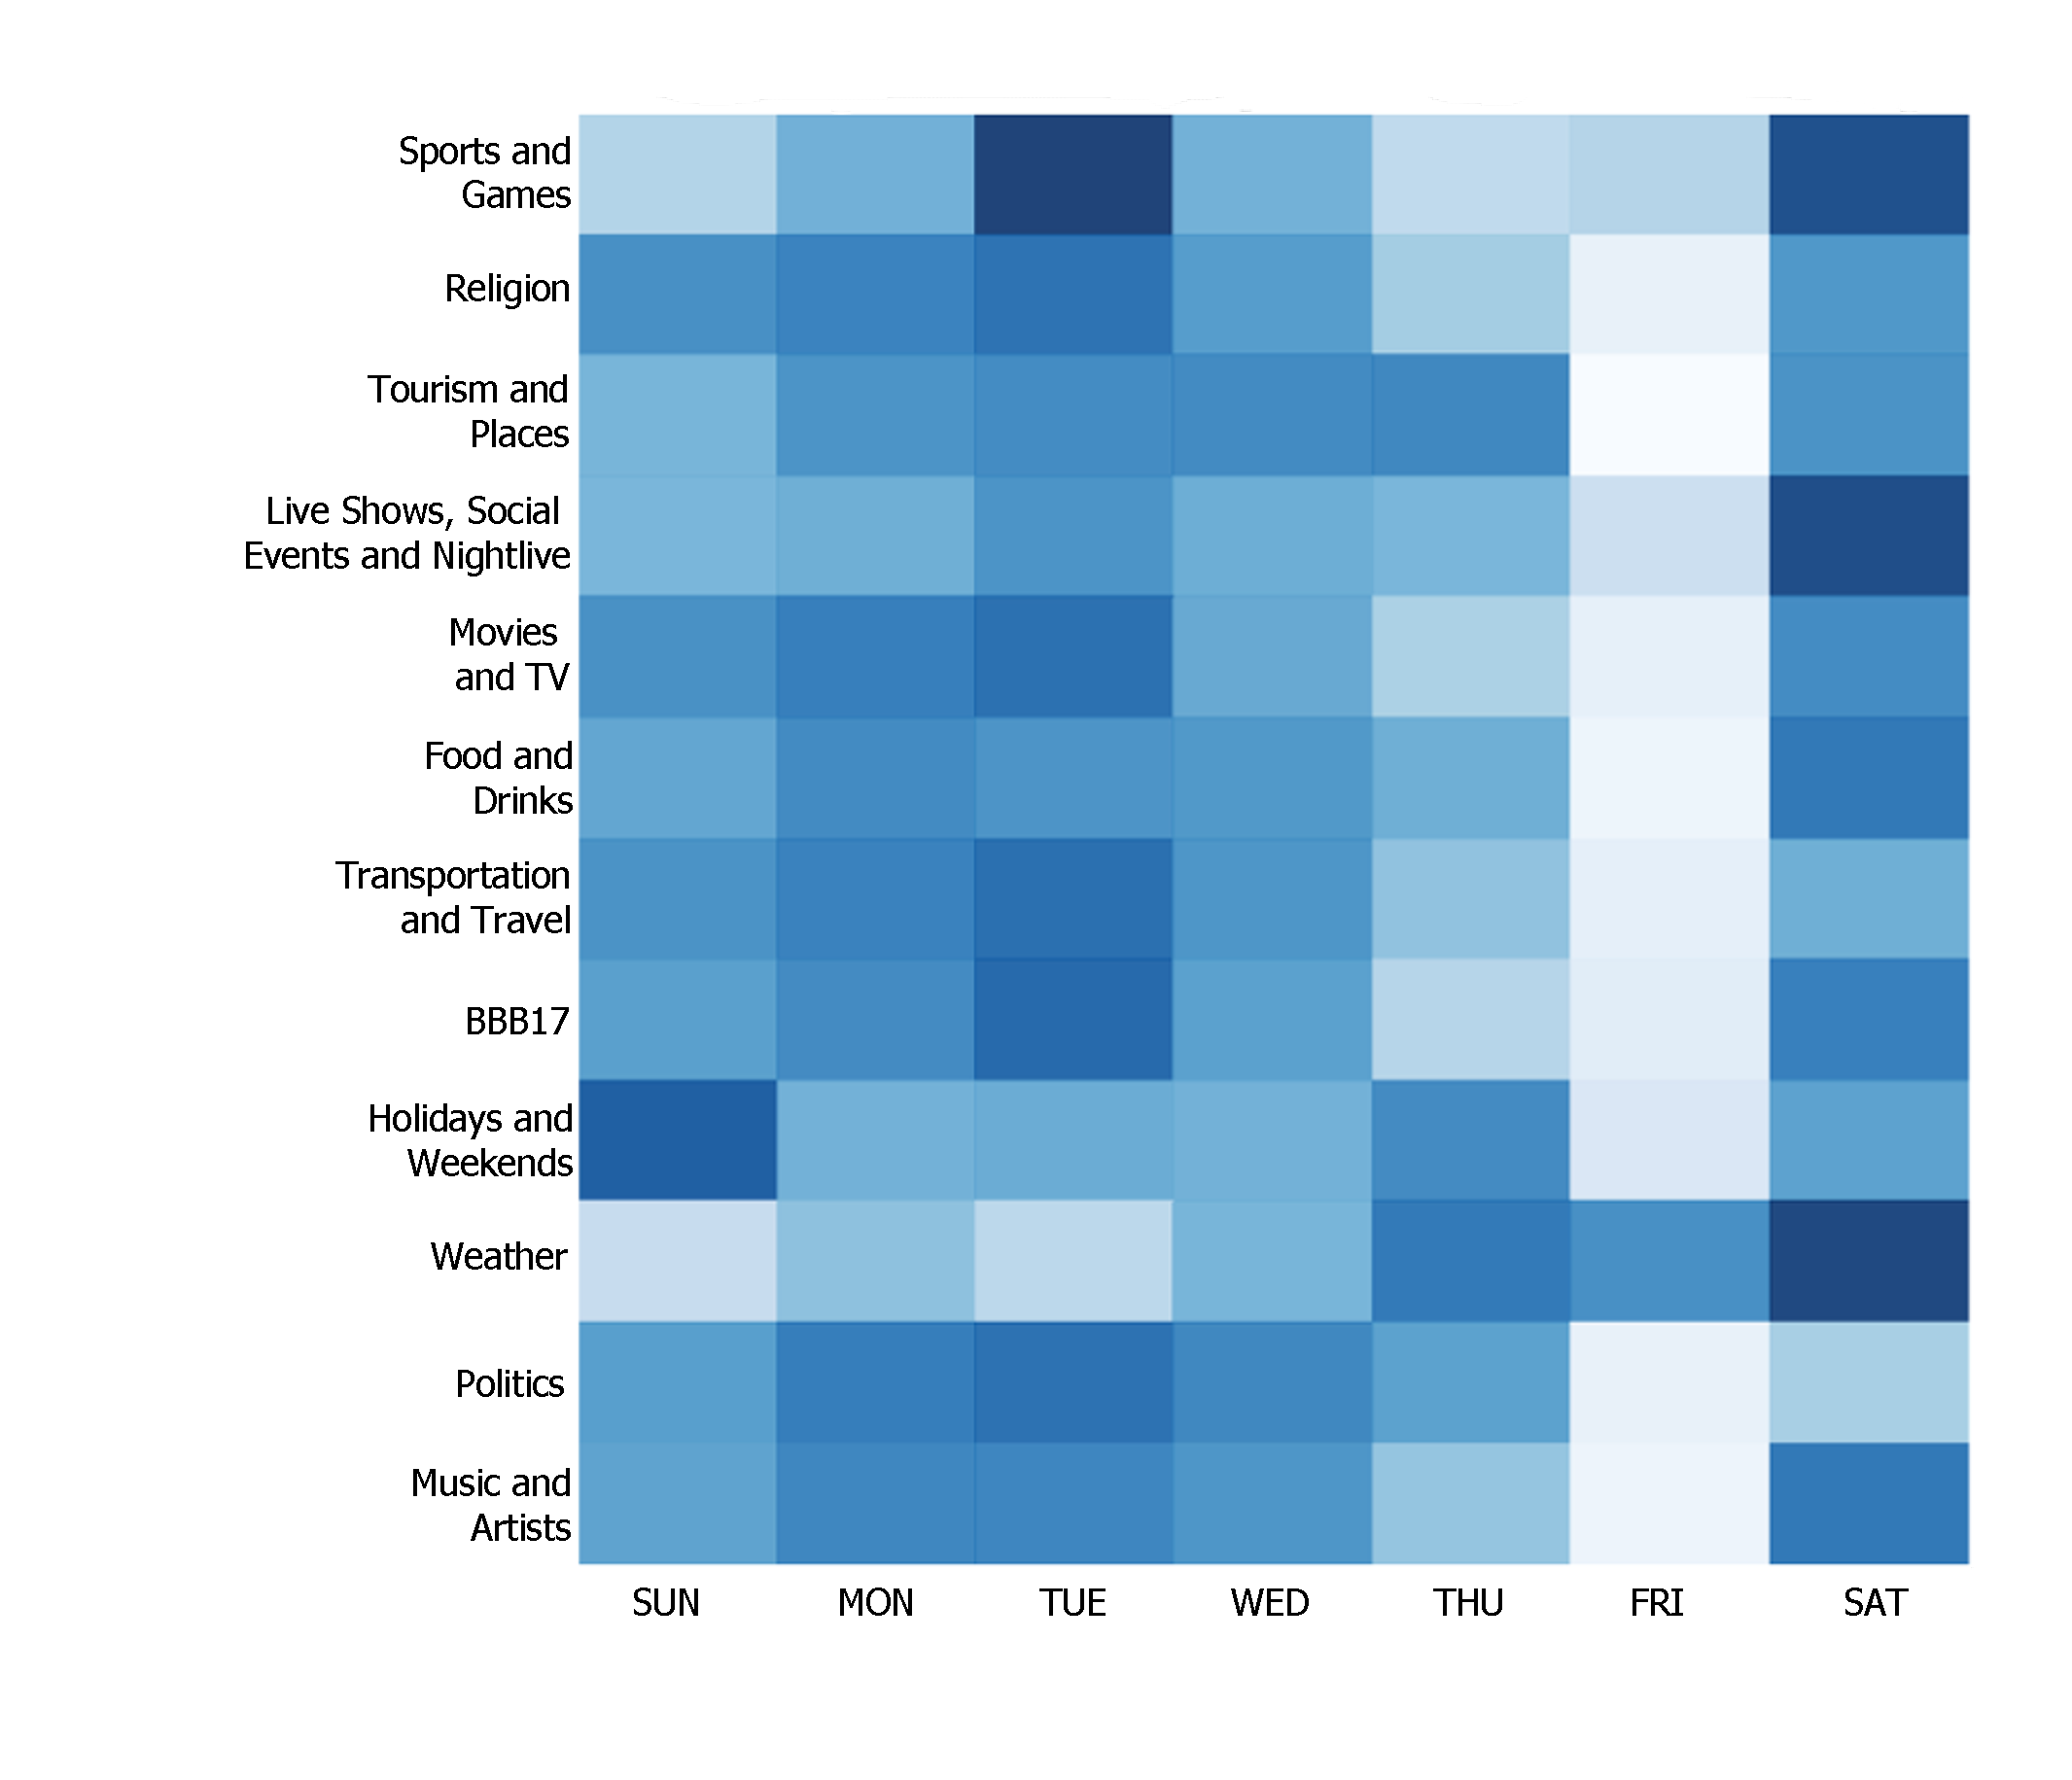
\includegraphics[width=1.0\linewidth]{figures/rio_topics_heatmap.pdf}
		\caption{Rio de Janeiro}
		\label{fig:rio}
	\end{subfigure}
	\begin{subfigure}{0.49\textwidth}
		\centering
		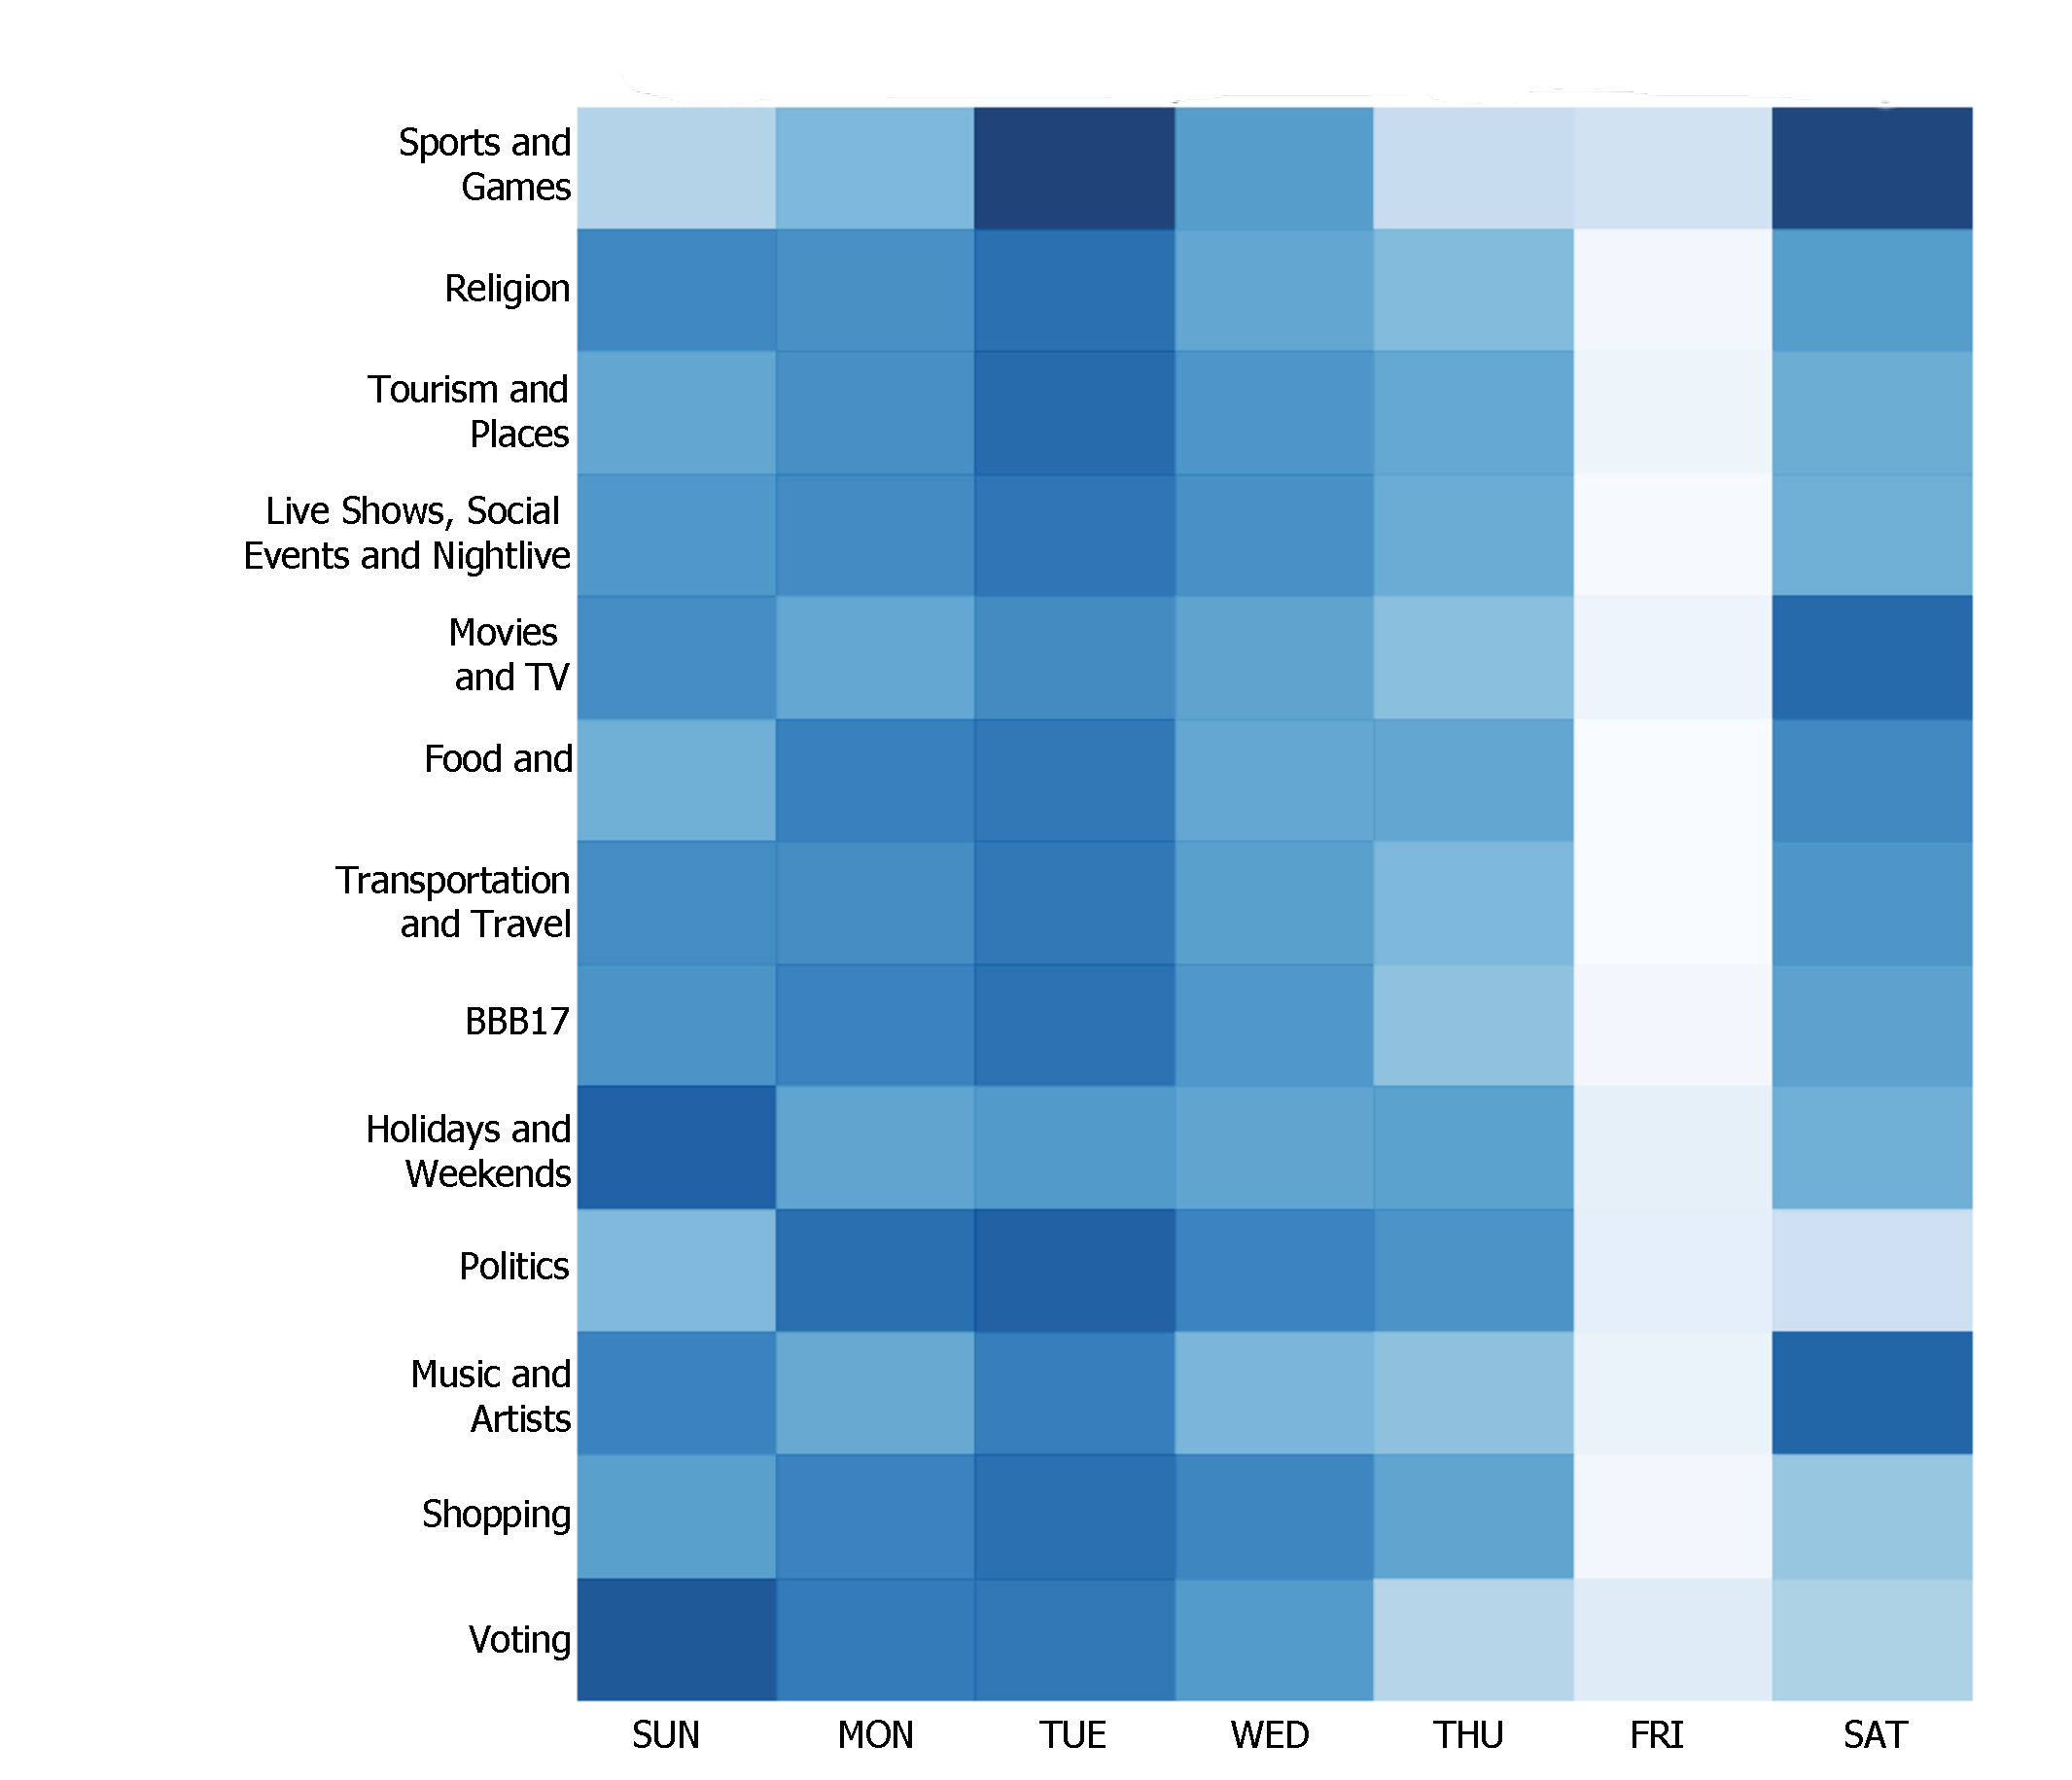
\includegraphics[width=1.0\linewidth]{figures/sp_topics_heatmap.pdf}
		\caption{São Paulo}
		\label{fig:sp}
	\end{subfigure}
	\caption[Day-of-the-week Twitter activity]{Day-of-the-week activity per each topic in both cities}
	\label{fig:topics_heat_maps}
\end{figure}

Only 12 topics of the finals 29 were selected for this part of the study, predicting them and comparing the final results, such as, but not limited to, \textit{Sports and Games}, \textit{Religion}, \textit{Holidays and Weekends}, \textit{Movies and TV}, \textit{Live Shows, Social Events and Nightlife}. The temporal distribution is showed in Figure~\ref{fig:topics_heat_maps} as a heat map, where each row is independent from the others.

The necessity of applying such restrictions is due to the need of seeing in which days each topic is more talked about. For both cities the topic \textit{Sports and Games} is more mentioned in Tuesdays and Saturdays. Indeed, this observation correlates with the days that topic-related events happens. Namely, Tuesdays and Wednesday correspond to the days when the \textit{UEFA Champions League} competition happens and Saturdays and Sundays to the days of \textit{Brazilian Football League} games. \textit{Holidays and Weekends} was a topic with interesting results regarding the temporal distribution, presenting Sundays as the day where more people talk about it. 

Furthermore, it is worth mentioning that our model had successfully discover a topic related to Big Brother Brazil 2017 (BBB17), a well-known reality show. The amount of geo-located tweets concerning this topic was considerable (1.85\% and 2.49\%, in RJ and SP, respectively), rising the question about what led people to geo-located them in such topic.

\subsection{Final Remarks}
This experiment demonstrates the capability of our framework to handle different topic modelling analysis under unregulated and non-conventional data such as the content found in most social media. The application of topic modeling technique to tweets from two different cities enables interesting comparisons between them since the whole analytics process accounts for what inhabitants talk about in their social networks. Through these analysis, cities' services are capable of monitoring human behaviour, activity patterns as well as of identifying regions where there may be some levels of intolerance on certain topics, making it possible to trigger preventive measures to solve problems in those specific areas.

LDA models usually require documents of large size, or at least ones with higher complexity than a single tweet so as to yield appropriate performance. A traditional approach was followed considering each tweet as a document instead of trying to aggregate tweets in more complex documents taking into consideration some criteria, e.g. grouping messages by date and hour. All topics resulting from our approach are similar in both cities but two, which are unique for each of the selected scenarios. The percentage difference between similar topics was within the interval 0.16-4.43\% evidencing the fact that both cities are also similar besides different factors that characterize each other: population, culture, lifestyle and also the region where the city is located in.

In spite of the analysis carried out and reported in this paper, we can not assure that inside a topic other encapsulated topics might exist. The resulting amount of tweets for each topic was extremely high, turning a one-by-one verification into a very laborious and time consuming process. Therefore, our classification approach was limited to the verification of the top-50 words and the manual identification of such words in samples of 200 tweets per topic. Such a limitation, nonetheless, did not prevent us to draw important conclusions relatively to the results we have obtained after the application of our proposed solutions, as discussed in the Section \ref{sec:results}.

Future direction for this research will include application of spatio-temporal aggregation methods over both datasets in order to create more complex documents and verify whether results can be different taking into consideration temporal and spatial factors. To pursue this, it is required that a large dataset for both cities is available, which is expectable only in mid- to long-term. A possible future evaluation approach to be considered is the mapping of topics over specific areas of the cities, such as the identification of topics related to beaches alongside the coastal area in Rio de Janeiro, or the identification of transportation and travel topics over the metropolitan area in São Paulo. Finally, it is also necessary to explore other classification/evaluation approaches to enhance robustness, consistency, and efficiency of the topic modelling routine; one possible solution is the method aforementioned in Section~\ref{related_work}, which considers the addition of an extra layer to endow the framework with supervised labeling capabilities.

\section{Travel-related Classification}
\label{sec:travel_related_classification}
The main goal of this section is to describe the experiments conducted to discriminate travel-related tweets in Rio de Janeiro, São Paulo and New York City. Considering the volume of the collected data for each scenario, it is necessary to automatically identify tweets whose content somehow suggests to be related to the transportation domain. Conventional approaches would require us to specify travel-related keywords to classify such tweets. On the contrary, our approach consisted in training a classification model to automatically discriminate travel-related tweets from non-related ones. 

One big challenge always present in text analysis is the sparse nature of data, which is especially the case in Twitter messages. Conventional techniques such as bag-of-words tend to produce sparse representations, which become even worse when data is composed by informal and noisy content.

Word embeddings, on the other hand, is a text representation technique that tries to capture syntactic and semantic relations from words. The result is a more cohesive representation where similar words are represented by similar vectors. For instance, \emph{"taxi"/"uber"}, \emph{"bus/busão/ônibus"}, \emph{"go to work"/"go to school"/"ir para a escola"} would yield similar vectors respectively.
We are particularly interested in exploring the characteristics of word embeddings techniques to understand which extent it is possible to improve the performance of our classifier to capture such travel-related expressions. In the reminder subsections, we describe two different text classification experiments following distinct approaches across two speaking languages - Portuguese and English.

Support Vector Machines (SVM), Logistic Regression (LR) and Random Forests (RF) were the classifiers used in these experiments. The SVM classifier was tested under three different kernels, namely \textit{rbf}, \textit{sigmoid} and \textit{linear}; the latter proved to obtain the best results for both experiments. 

The LR classifier was used with the standard parameters, whereas the RF classifier used 100 trees in the forest. The gini criterion and the maximum number of features were limited to those as aforementioned in Section~\ref{sec:travel_features}, in the case of the RF classifier.

To evaluate the performance of classifiers in our experiences we used five different metrics. Firstly we compute a group of three per-class metrics, namely precision, recall and the F1-score. Bearing in mind this study considers a binary classification, metrics were associated with the travel-related class only, i.e. the positive class.

We established the use of different groups of features to train our classification model, namely bag-of-words, bag-of-embeddings - word embeddings dependent technique - and both combined (horizontally combination of bag-of-words and bag-of-embeddings matrices into a single one).

\subsection{Rio de Janeiro and São Paulo}
\label{subsec:rio_de_janeiro_sao_paulo_experiment}

Messages were collected for a period of a whole month, between days March 12 and April 12, 2017, and the resulting datasets sum up a total of 6.1M and 2.9M tweets for Rio de Janeiro and São Paulo, respectively. Due to the problem detected in Section~\ref{sec:geographical_distribution}, we filtered the data in order to use only tweets that were actually inside the cities' areas. The final composition of the datasets is presented in Table~\ref{tab:brazilian_datasets_travel}, and the subset of data considered in this experiment sum up a total of 7.7M tweets -  5.3M and 2.4M tweets for Rio de Janeiro and São Paulo, respectively.

\begin{table}[ht]
	\small
	\centering
	\caption{Portuguese datasets composition for the travel-related classification experiment}
	\label{tab:brazilian_datasets_travel}
	\resizebox{\textwidth}{!}{\begin{tabular}{|c|c|c|c|c|c|c|}
			\hline
			\textbf{City}  & \textbf{All} & \textbf{PT} & \textbf{Non-PT} & \textbf{\begin{tabular}[c]{@{}c@{}}Inside \\ Bounding-Box\end{tabular}} & \textbf{\begin{tabular}[c]{@{}c@{}}Outside\\ Bounding-Box\end{tabular}} & \textbf{\begin{tabular}[c]{@{}c@{}}PT and Inside \\ Bounding-Box\end{tabular}} \\ \hline
			Rio de Janeiro & 6,175,000 & 5,355,000 & 819,000 & 4,327,000 & 1,848,000 & 3,749,000 \\ \hline
			São Paulo      & 2,934,000 & 2,444,000 & 490,000 & 2,016,000 & 918,000 & 1,672,000 \\ \hline
		\end{tabular}}
	\end{table}

\subsubsection{Training and Test Datasets}
\label{subsec:training_test_datasets_portuguese}
The construction of the training and test sets followed a semi-automatic labeling approach. We tried to built a balanced training set concerning the travel-related class and the non-related. The selection process of tweets have support on a strategy used in the study of Maghrebi et al.~\cite{maghrebi2016transportation}, which consists in searching tweets from a collection using specific travel terms in conjecture with white-spaces in the start and end of a regular expression (e.g. \emph{" carro "}, for the car mode of transport). Using the terms declared in Table~\ref{tab:terms} combined with the previous mentioned regular expression, we found about 30,000 tweets. From this subset, we randomly selected a small sample of 3,000 tweets to manually confirm if they were indeed related to travel topics. Although the randomly selection of tweets to produce such training set, we careful analyse the existence of all modes of transportation present in Table~\ref{tab:terms}. After this manual annotation we selected 2,000 tweets and used them as positive samples in the training dataset.

\begin{table}[htbp]
	\centering
	\small
	\caption{Travel terms used to build the training set}
	\label{tab:terms}
	\begin{tabular}{c|c|c}
		\hline
		\multirow{2}{*}{\textbf{Mode of Transport}} & \multicolumn{2}{c}{\textbf{Terms}} \\ \cline{2-3} 
		& \multicolumn{1}{l|}{\textbf{Portuguese Language}} & \textbf{English Language} \\ \hline
		\textbf{Bike} & bicicleta, moto & bicycle, bike \\
		\textbf{Bus} & onibus, ônibus & bus \\
		\textbf{Car} & carro & car \\
		\textbf{Taxi} & taxi, táxi & taxi, cab \\
		\textbf{Train} & metro, metrô, trem & metro, train, subway \\
		\textbf{Walk} & caminhar & walk \\ \hline
	\end{tabular}
\end{table}

In order to select negative samples for the training dataset we randomly selected 2,000 tweets and also manually verified their content to assure that they were not travel-related. Finally, our training set was composed by 4,000 tweets, from which 2,000 were travel-related and 2,000 were not. 
We selected 1,000 tweets randomly that were not present in the training set to build the test set, and then manually classified them as travel-related or non-travel-related. In the end, 71 tweets were found to be travel-related and whereas 929 were not.

It is worth mention that we try to hide some terms from the training set in order to verify if the embeddings were able to discriminate tweets about \emph{"Uber"/"Busão"}, which are terms related to the \texttt{car/taxi} and \texttt{bus} modes of transport, respectively. To assure such test, we incorporate specific-related tweets about these modes of transport in the 71 travel-related tweets of the test set. By obtaining good result regarding the performance of the classification model, we can induce several advantages regarding the use of word-embeddings-based features in social media classification tasks for a large diversity of domains, such as the smart cities and transportation domains.

\subsubsection{Results and Analysis}
\label{subsubsec:results_rio_de_janeiro_sao_paulo}
Table~\ref{classifiers} presents the results obtained using the different features combination for our test set composed by 1,000 tweets manually annotated. According to the evaluation metrics we conclude that the bag-of-word and bag-of-embeddings combined produced better classification models. The model produced by the Linear SVM performed slightly better than the LR and the RF. Interesting to note is that \gls{BoW} features have influence on the precision scores obtained from our results, producing more conservative classifiers. Regarding the recall results, we can see that the Logistic Regression using only bag-of-embeddings features was the model with best results; perhaps if the precision is taken into consideration, the same conclusions will not be possible. Analysing the scores provided in Table~\ref{classifiers}, the best model under the F1-score was the Linear SVM, with a score of 0.85. It is worth noting that combining Bag-of-words and Bag-of-embedding with size 100 was the group of features with best performance taking into consideration the evaluation metrics used in this experiment.

\begin{table}[!bp]
	\small
	\centering
	\caption{Performance results with 100 sized vectors for BoE}
	\label{classifiers}
	\begin{tabular}{c|c|c|c|c}
		\hline
		\textbf{Classifier}                  & \textbf{Features} & \textbf{Precision} & \textbf{Recall} & \textbf{F1-score} \\ \hline
		\multirow{3}{*}{Linear SVM}          & BoW               & 1.0                & 0.6761          & 0.8067            \\
		& BoE               & 0.4338             & 0.8309          & 0.5700            \\
		& \textbf{BoW + BoE}         & \textbf{1.0}       & \textbf{0.7465} & \textbf{0.8548}   \\ \hline
		\multirow{3}{*}{Logistic Regression} & BoW               & 1.0                & 0.6338          & 0.7759            \\
		& BoE               & 0.4444             & 0.8451          & 0.5825            \\
		& BoW + BoE         & 1.0                & 0.6761          & 0.8067            \\ \hline
		\multirow{3}{*}{Random Forest}       & BoW               & 1.0                & 0.6338          & 0.7759            \\
		& BoE               & 0.2298             & 0.8028          & 0.3574            \\
		& BoW + BoE         & 1.0                & 0.6338          & 0.7759            \\ \hline
	\end{tabular}
\end{table}


\begin{figure}[!htp]
	\centering
	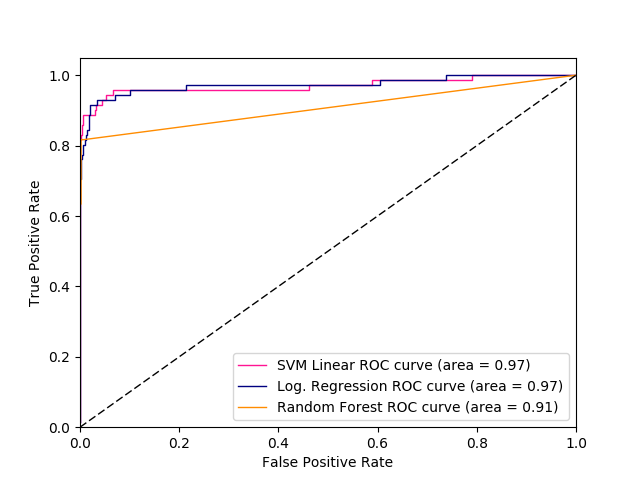
\includegraphics[width=0.7\textwidth]{figures/roc_auc_brazilian_travel_related}
	\caption{ROC Curve of SVM, LR and RF experiences}
	\label{fig:roc_curve}
\end{figure}

\begin{figure}[!hbp]
	\centering
	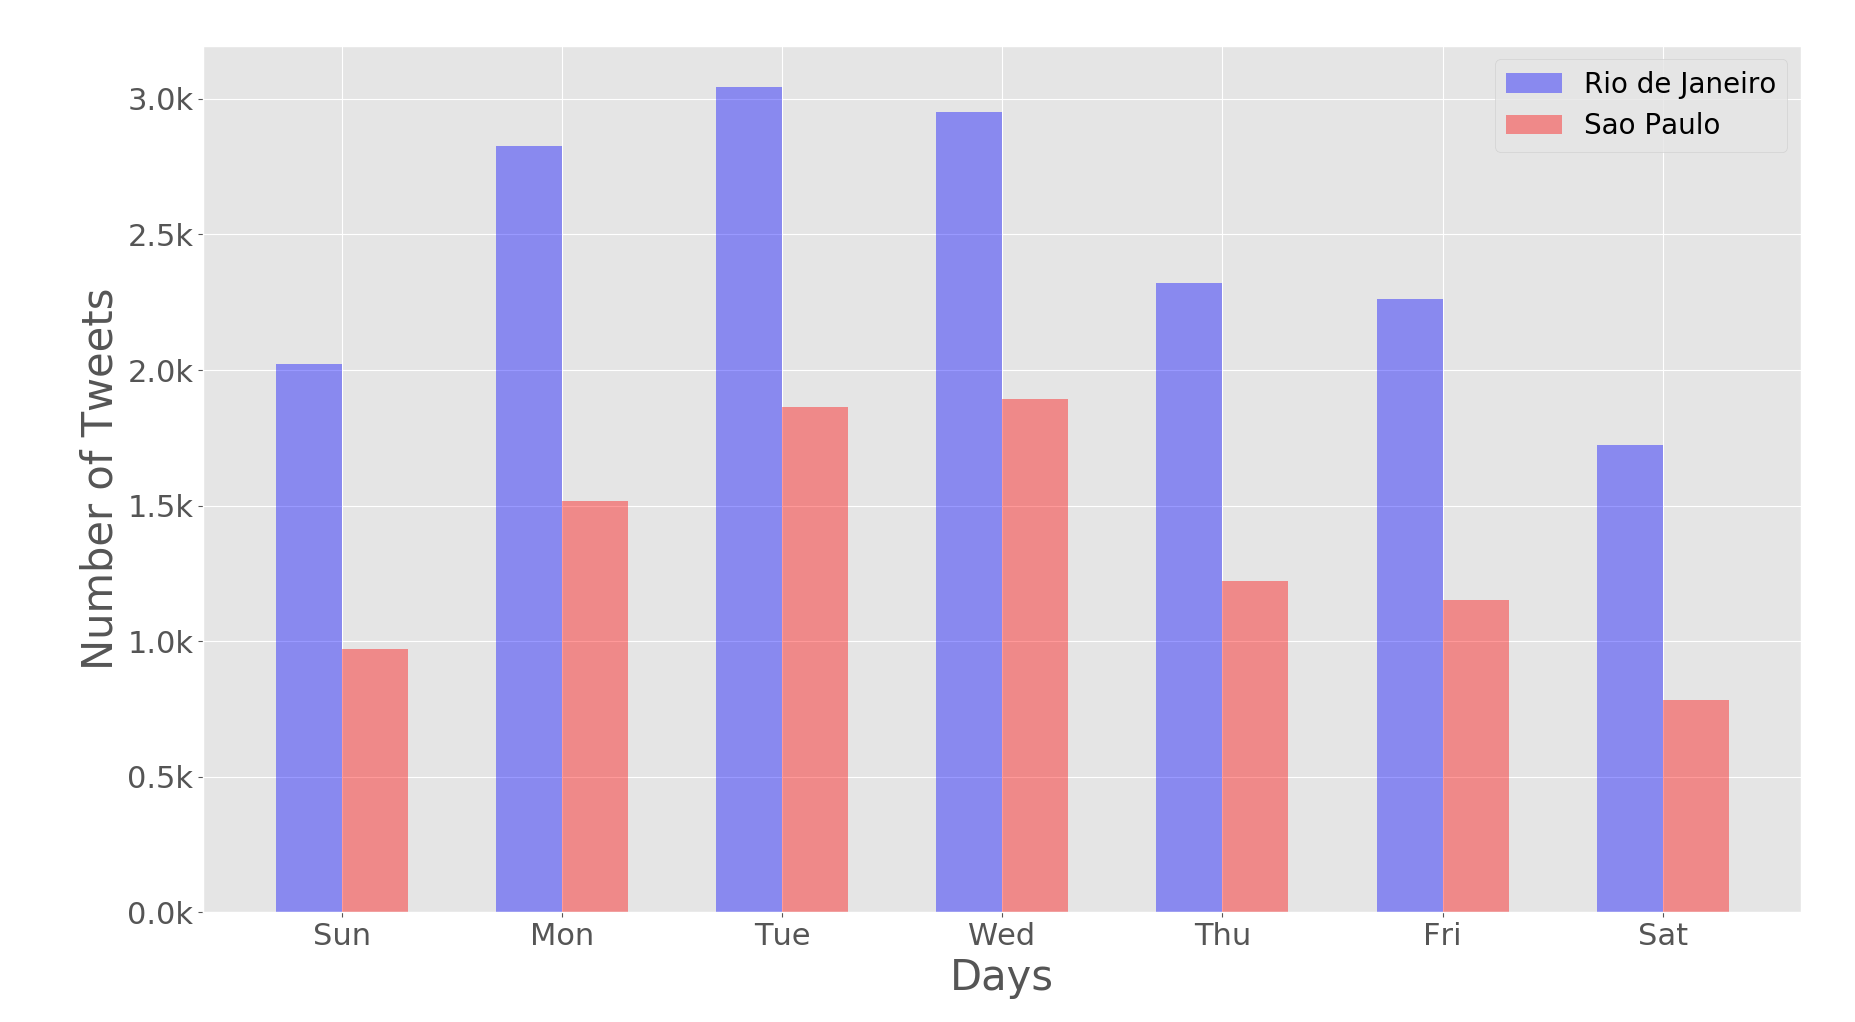
\includegraphics[width=0.7\textwidth]{figures/predicted_day_of_week}
	\caption{Positive Predicted Tweets per Day of Week}
	\label{fig:predicted}
\end{figure}


The performance of all three classifiers is illustrated using the ROC Curve in Figure~\ref{fig:roc_curve}.

The area under the curve of the Receiver Operating Characteristic (AUROC) was very similar for both the Logistic Regression and the Linear SVM models. The results obtained from the Random Forest model were not so promising as expected.

After the selection of our classification model, we decided to classify all the Portuguese dataset and draw some statistics from the results. The trained Linear SVM classifier was used to predict whether tweets were travel-related or not, since it was the model presenting the best score under the F1-score metric (as shown in Table~\ref{classifiers}). From a total of 7.8M tweets, our classifier was able identified 37,300 travel-related entries.

\begin{figure}[!bp]
	\centering
	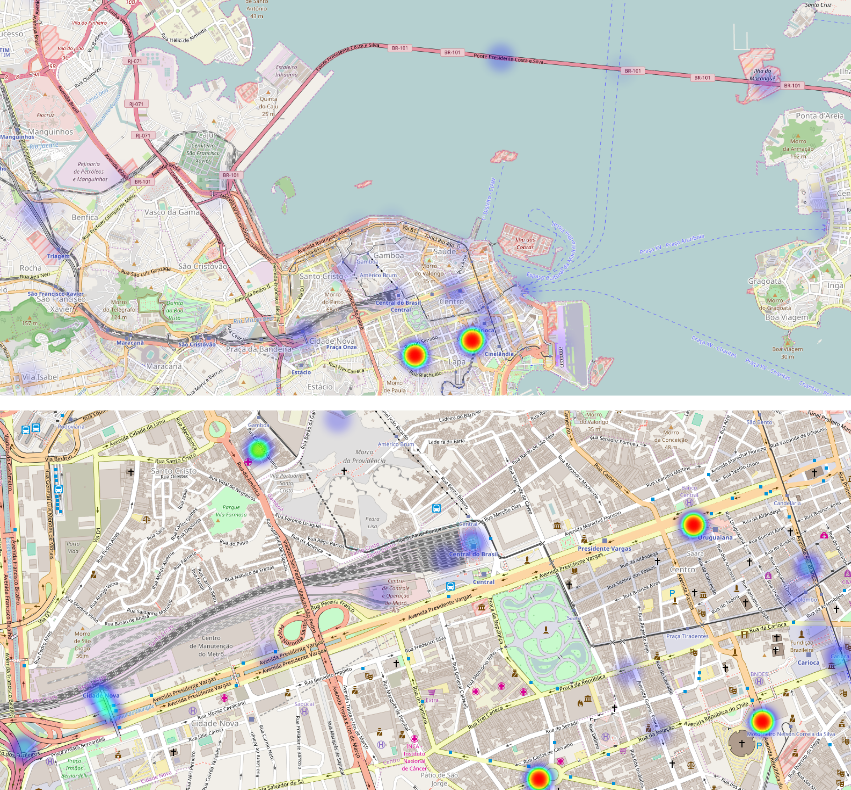
\includegraphics[width=0.7\textwidth]{figures/rio_1}
	\caption{Rio de Janeiro heat map to the positive tweets}
	\label{subfig:rio_heatmap}
\end{figure}

\begin{figure}[!htp]
	\centering
	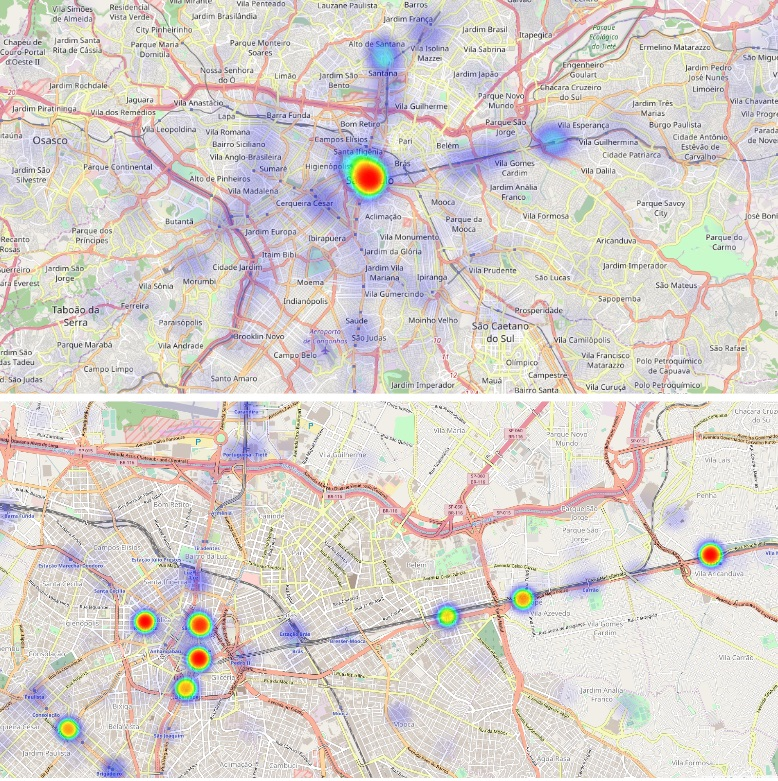
\includegraphics[width=0.7\textwidth]{figures/sp_1}
	\caption{São Paulo heat map to the positive tweets}
	\label{subfig:sp_heatmap}
\end{figure}

Figure~\ref{fig:predicted} depicts the distribution of travel-related tweets over the days of the week. We can see that the first three business days (Monday, Tuesday and Wednesday) are the ones on which the Twitter activity is higher for both cities in our study.

In order to understand the spatial distribution of travel-related tweets we generated a heatmap for both cities. From the heatmap of Rio de Janeiro, illustrated in Figure~\ref{subfig:rio_heatmap}, it is possible to identify that some agglomerations of tweets are located at Central do Brasil, Cidade Nova and Triagem train stations, as well as at Uruguaiana, Maracanã and Carioca metro stations. The Rio-Niterói bridge, connecting Rio de Janeiro to Niterói, as well as the piers on both sides also presented considerable clouds of tweets classified as travel-related.

The heatmap for the city of SP, illustrated in Figure~\ref{subfig:sp_heatmap}, was also an interesting case to observe. Almost every agglomeration matched some metro or train station. Estação Brás, Tatuapé, Belém, Estação Paulista, Sé, Liberdade were some of the stations highlighted in the heatmap. We could also identify a little agglomeration of travel-related tweets at Congonhas airport, even though no tweets seemed to mention the word \textit{plane} explicitly in the training of our classification model.

\subsubsection{Final Remarks}
The previous described experiment explores an approach of supervised learning using as training examples a set of manually annotated tweets extracted from the whole datasets with the support of a term-based regular expression. The overall methodology is concerned with the problem of construct a fine-grained Twitter training set for the travel domain and also the automatic identification of travel-related tweets from a large scale corpus. We combined different word representations to verify whether our classification model could learn relations between words at both syntactic and semantic levels. After using standard techniques such as bag-of-words and bag-of-embeddings, we have used them combined yielding results that showed that these different groups of features can complement each other, with respect to Portuguese-speaking tweets. Modes of transport are always evolving and new services emerges making the identification of tweets related to it difficult. Overall, our experiment proved that word-embeddings features are actually an advantage regarding its applicability into instable real-world scenarios such as the transportation domain. 

\subsection{New York City}
\label{subsec:new_york_city_experiment}

Similar to the experiment of Portuguese-speaking travel-related classification of tweets, we built a model to discriminate English-speaking travel-related tweets. However, the construction of the training and test sets in this experiment follows a different approach. While in the Rio de Janeiro and São Paulo experiment we explore an semi-automatic approach and tweets were almost instantaneous formed as a group, here we were obligate to follow a two-phase approach due to the polysemy level of English travel terms.

Differently from the Brazilian cities experiment, tweets were collected from New York City during a period of two months, between days March 12 and May 12, 2017. Ignoring all non-English, as well as tweets located outside the bounding-box of New York City, the resulting dataset comprehends 4M tweets.

Regarding the preparation of data, we used the same preprocessing operations in both experiments, Brazilian and North-American. The operations were lowercasing, transformation of repeated characters and cleaning of \emph{entities} (user mentions and URLs) from the message content.

\subsubsection{Training and Test Datasets}

In the Portuguese dictionary, travel-related terms do not have more than one meaning. For instance \emph{"caminhar"} or even \emph{"comboio"} possesses only one meaning. Regarding the English dictionary, travel-related tweets may have more than one meaning since some of them present high level of polysemy. Terms such as \emph{"walk"} may be used to describe the action of walk or, for example, the action of \emph{walk into}. On the other hand, the term \emph{"train"} can be used to describe the mode of transport train or a type of behaviour through practice and instruction.

The polysemy level of such terms was took into consideration while the construction process of our training set of tweets for the English-language travel-related classification model. In the first stage of the construction process, we used the same strategy of the Portuguese training set. By take support on a semi-automatic labeling technique using a regular expression, we find out almost 16,000 tweets. The next step in the construction process was a manually verification followed by a manually annotation. Overall, 1,686 tweets were selected for each of both binary classes, travel-related and non-related. The travel-related set was strictly balanced in order to have almost the same amount of examples for each of the travel-modes involved in this study. The non-related training set is composed of several subjects that are not related to travel, e.g. football, leisure, politician, personal tweets, among others.

Nonetheless, we include into the training set tweets which polysemy level may induce doubts regarding the context of the message in order to make possible higher levels of discrimination in our model. This inclusion may help the learning process of our model making it capable of correctly identify which are the tweets that are actually related to the travel and transportation domain.
The final composition of the training datasets is presented in Table~\ref{tab:new_york_first_dataset}.

\begin{table}[!tp]
	\centering
	\caption[English-speaking tweets datasets]{Composition of the training and test datasets for the English travel-related tweets classification}
	\label{tab:new_york_first_dataset}
	\begin{tabular}{c|c|c|}
		\cline{2-3}
		\textbf{}                                       & \multicolumn{2}{c|}{\textbf{Training Set}}                          \\ \hline
		\multicolumn{1}{|c|}{\textbf{Mode of Tranport}} & \textbf{Travel-related} & \multicolumn{1}{l|}{\textbf{Non-related}} \\ \hline
		\multicolumn{1}{|c|}{Bike}                      & 300                     & \multirow{6}{*}{1686}                     \\
		\multicolumn{1}{|c|}{Bus}                       & 311                     &                                           \\
		\multicolumn{1}{|c|}{Car}                       & 317                     &                                           \\
		\multicolumn{1}{|c|}{Taxi}                      & 314                     &                                           \\
		\multicolumn{1}{|c|}{Train}                     & 317                     &                                           \\
		\multicolumn{1}{|c|}{Walk}                      & 217                     &                                           \\ \hline
		\multicolumn{1}{|c|}{\textbf{Total}}            & \multicolumn{2}{c|}{3372}                                           \\ \hline
	\end{tabular}
\end{table}

\subsubsection{Preliminary Results}\label{subsec:preliminar_results}
Due to the laborious and time-consuming effort made in the construction of the training set, we opt to apply a different approach in the training phase of our model classification model. In order to enhance the differences between tweets whose terms present high levels of polysemy, the model was trained using a \gls{k-fold-cross-validation} technique with 10 iterations for all groups of features: bag-of-words and bag-of-embeddings and both combined. Results showed good performance for all models regarding the selected evaluation metrics. The best model in this experiment was the Logistic Regression classifier trained with bag-of-words and bag-of-embeddings features, presenting a F1-score of 0,98324.

\begin{table}[!bp]
	\centering
	\caption[New York City First Experiment Results]{Preliminary results (it is only demonstrated the best result for the bag-of-embeddings group)}
	\label{tab:first_experiment}
	\begin{tabular}{|c|c|c|c|c|}
		\hline
		\textbf{Classifier} & \textbf{Features} & \textbf{Precision} & \textbf{Recall} & \textbf{F1-score} \\ \hline
		\multirow{3}{*}{\textbf{Linear SVM}} & BoE(200) & 0,90883 & 0,83634 & 0,87089 \\
		& BoW & 0,96298 & 0,97652 & 0,96962 \\
		& \textbf{BoE(200) + BoW} & \textbf{0,97251} & \textbf{0,99114} & \textbf{0,98170} \\ \hline
		\multirow{3}{*}{\textbf{Logistic Regression}} & BoE(100) & 0,90172 & 0,84948 & 0,87447 \\
		& BoW & 0,96431 & 0,98042 & 0,97222 \\
		& \textbf{BoE(200) + BoW} & \textbf{0,97391} & \textbf{0,99285} & \textbf{0,98324} \\ \hline
		\multirow{3}{*}{\textbf{Random Forests}} & BoE(100) & 0,81283 & 0,83600 & 0,82394 \\
		& BoW & 0,96569 & 0,98997 & 0,97764 \\
		& \textbf{BoE(50) + BoW} & \textbf{0,93688} & \textbf{0,99939} & \textbf{0,96701} \\ \hline
	\end{tabular}
\end{table}

The fact that all models performed incredibly well, in particular models using the features group of \gls{BoW} and \gls{BoW}+\gls{BoE} raise to us some questions and doubts about the robustness of the features used in the training process. First, in the Brazilian cities experiment, by following the same approach over the training set construction process we did not obtain results of this kind. Second, the selected tweets are very specific and our model may be overfitted due to training data. In order to pursue and have answers to our questions, we designed another experiment using the same dataset.

\iffalse
\begin{table}[htbp]
	\small
	\centering
	\caption{Preliminary Results}
	\label{tab:first_experiment}
	\begin{tabular}{|c|c|c|c|c|}
		\hline
		\textbf{Classifier} & \textbf{Features} & \textbf{Precision} & \textbf{Recall}  & \textbf{F1-score} \\ \hline
		\multirow{2}{*}{\textbf{Linear SVM}} & BoE (200) & 0,90883   & 0,83634 & 0,87089  \\
		& \textbf{BoW} & \textbf{0,96298}   & \textbf{0,97652} & \textbf{0,96962}  \\ \hline
		\multirow{2}{*}{\textbf{Logistic Regression}} & BoE (100) & 0,90172   & 0,84948 & 0,87447  \\
		& \textbf{BoW} & \textbf{0,96431}   & \textbf{0,98042} & \textbf{0,97222}  \\ \hline
		\multirow{2}{*}{\textbf{Random Forests}} & BoE (100) & 0,81283   & 0,83600 & 0,82394  \\
		& \textbf{BoW} & \textbf{0,96569}   & \textbf{0,98997} & \textbf{0,97764}  \\ \hline
	\end{tabular}
\end{table}
\fi

\subsubsection{\emph{Leave-one-group-out}}\label{subsec:leave_one_group_out}

It is worth noting that in our first experiment all travel-mode classes were known by the model before the classification of the test set (the remaining sub-dataset in the 10-fold cross-validation). Comparing with real-world scenarios, this may not be true since new modes of transport and companies, such as Uber, Lyft and Cabify, arise from unpredictable moments. This second experiment follows a \emph{leave-one-group-out} strategy, meaning that one travel-mode class if left out of the training set and moved into the test set. Hence, the behaviour of the learned model when facing a completely unknown travel-mode class can be evaluated. A model for each hidden transport-mode class was built and evaluated using the same training conditions and metrics. The datasets composition of each experiment led in this strategy can be observed in Table~\ref{tab:leave}.

\begin{table}[htbp]
	\small
	\centering
	\caption[\emph{Leave-one-group-out expirement datasets}]{Datasets composition used in the \emph{leave-one-group-out} strategy}
	\label{tab:leave}
	\begin{tabular}{|c|c|c|c|c|}
		\hline
		\multirow{2}{*}{\textbf{\begin{tabular}[c]{@{}c@{}}Travel-Mode \\ Class\end{tabular}}} & \multicolumn{2}{c|}{\textbf{Training Set}} & \multicolumn{2}{c|}{\textbf{Test Set}} \\ \cline{2-5} & \textbf{Pos.} & \textbf{Neg.} & \textbf{Pos.}  & \textbf{Neg.}  \\ \hline
		Taxi & 1,372 & \multirow{6}{*}{1,686}   & 314 & \multirow{6}{*}{300}  \\
		Train & 1,369 & & 317 & \\
		Car  & 1,369 & & 317 & \\
		Bike & 1,386 & & 300 & \\
		Walk & 1,469 & & 217 & \\
		Bus  & 1,375 & & 311 & \\ \hline
	\end{tabular}
\end{table}

For each experiment of the learning models, we maintain a 10-fold cross-validation approach, however it was built a test set with a hidden travel-mode class and 300 non-related tweets (negative class). Here, only bag-of-words and bag-of-embeddings features were fed into our models classification routine since the main goal of this experiment is to check the features robustness. Table~\ref{tab:results} presents the best results for each model, as so the group of features feeding it. To achieve the final results of this experiment, we calculated the mean between all models' results to each of the hidden transport-mode classes.

\begin{table}[!bp]
	\small
	\centering
	\caption{\emph{Leave one group out} experiments results for SVM, LR and RF classifiers}
	\label{tab:results}
	\begin{tabular}{|c|c|c|c|c|}
		\hline
		\textbf{Classifier} & \textbf{Features}  & \textbf{Precision} & \textbf{Recall}  & \textbf{F1-score} \\ \hline
		\multirow{2}{*}{\textbf{Random Forests}} & BoW & 0,40774 & 0,07474 & 0,12629  \\
		& \textbf{BoE (50)}  & \textbf{0,80278} & \textbf{0,76194} & \textbf{0,78447}  \\ \hline
		\multirow{2}{*}{\textbf{Logistic Regression}} & BoW & 0,40774 & 0,07474 & 0,12629  \\
		& \textbf{BoE (50)}  & \textbf{0,84882} & \textbf{0,75702} & \textbf{0,80219}  \\ \hline
		\multirow{2}{*}{\textbf{Linear SVM}} & BoW & 0,41527 & 0,07153 & 0,12203  \\
		& \textbf{BoE (200)} & \textbf{0,86374} & \textbf{0,75715} & \textbf{0,81289}  \\ \hline
	\end{tabular}
\end{table}

According to results, all classification models have performed reasonably well under the bag-of-embeddings features group, although the dimensionality used being different for the Linear SVM classifier.

After testing each model with a hidden travel-mode class, the models trained with bag-of-words features demonstrated poor performance when facing unknown travel-modes, revealing higher sensitivity and lower generalization capabilities in comparison to the bag-of-embeddings version. The generalization power is an important and crucial characteristic for our desired solution since in a real world scenario is very likely that we will face a higher variety of categories that were not taken into consideration in the training phase of our model. Having this considered, the bag-of-words features group presents lack of robustness as we doubt in our first experiment (Section~\ref{subsec:preliminar_results}).

\begin{figure}[htbp]
	\centering
	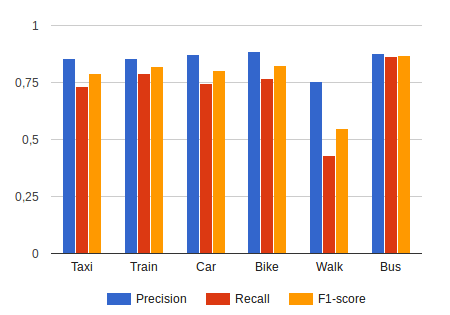
\includegraphics[scale=0.7]{figures/svm_linear_leave_one_out_emb_200.png}
	\caption{SVM model with BoE(200) for each travel mode}
	\label{fig:svm_leave}
\end{figure}

The best result of the \emph{leave-one-group-out} was the Linear SVM model, with the dimensionality of 200 in the size of the feature vectors. Figure~\ref{fig:svm_leave} presents the results of each experiment led for the different hidden travel-mode classes. An interesting point to observe is the low performance obtained to the experiment with the travel-mode class "Walk" hidden. This is due to the different semantic and syntactic contexts that the word \emph{walk} is used. Although all other classes can be used in the same context, for example, \emph{car}, \emph{train}, or \emph{bus}, usually the word \emph{walk} is not applied in the same way.

Having the experiments concluded, we used the best model, in this case, Linear SVM for the dimensionality of 200, to predict the 4M tweets that composed the NYC dataset. Almost 300,000 tweets were classified as travel-related. After the classification step, a sample of 10,000 tweets was taken from all the travel-related classified tweets and it was produced a heat-map distribution in order to verify which are the most concentrated zones. Such distribution enables the identification of associations with metro, train, bus stations. In Figure~\ref{fig:brooklyn}, that shows the south of the Manhattan island and also the Brooklyn bridge, it is possible no note some agglomerations over the bridge and also in the port and closed to the Wall Street(4.5) where there are some metro stations. The Central Park is one place that also took our attention since presented several agglomerations of tweets. In this particular place, tweets related to the walk class were correctly identified.

\begin{table}[htbp]
	\centering
	\small
	\caption{Sample of tweet messages correctly classified}
	\label{tab:tweets_examples}
	\resizebox{\textwidth}{!}{\begin{tabular}{|c|}
			\hline
			when you get into your uber and he has a pipe in the back \\
			a ground stop for \#ewr is no longer in effect \#flightdelay \\
			snowy walk to work. \#blizzard2017 \#centralpark \#noreaster2017 \@ bethesda terrace fountain -  \textbf{Figure~\ref{fig:central_park}} \\
			m.t.a. n.y.c subways: w train irregular subway service at whitehall street-south ferry \#traffic - \textbf{Figure~\ref{fig:brooklyn}} \\ \hline
		\end{tabular}}
	\end{table}

\begin{figure}[htbp]
	\centering
	\begin{subfigure}[htbp]{0.7\textwidth}
		\centering
		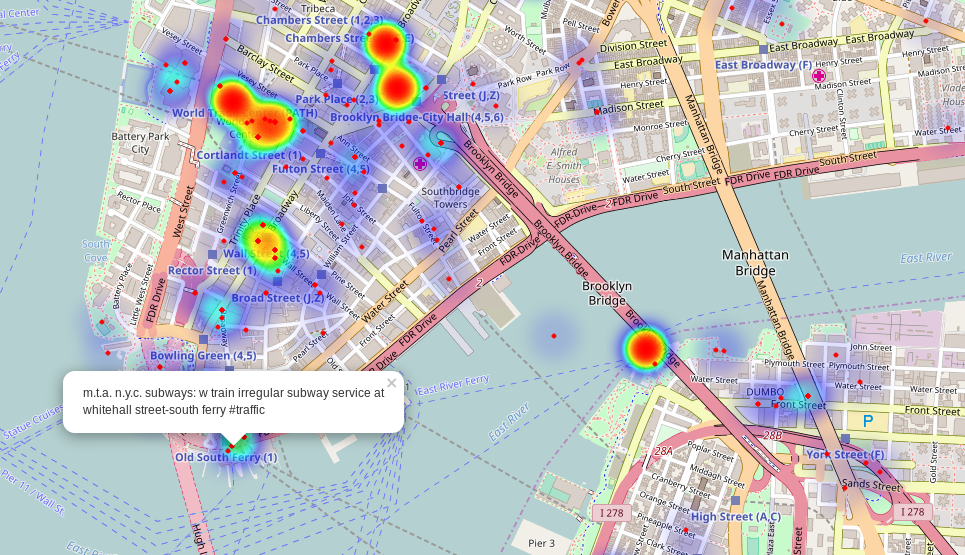
\includegraphics[width=0.9\columnwidth]{figures/nyc_map.png}
		\caption{}
		\label{fig:brooklyn}
	\end{subfigure}
	
	\medskip
	
	\centering
	\begin{subfigure}[htbp]{0.7\textwidth}
		\centering
		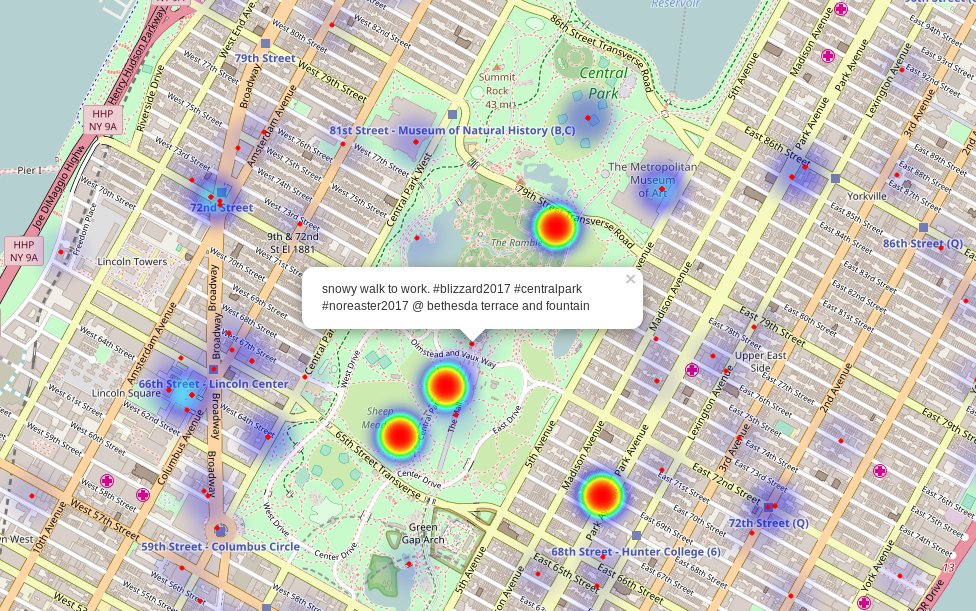
\includegraphics[width=0.9\columnwidth]{figures/nyc_map2.png}
		\caption{}
		\label{fig:central_park}
	\end{subfigure}
	
	\caption[Spatial density of the predicted tweets]{Spatial density of the travel-related predicted tweets in New York City: (a) South of Manhattan and over the Brooklyn Bridge, (b) Central Park}
	\label{fig:nyc__geographical_distribution}
\end{figure}

\subsection{Concluding Remarks}
The main objective of this experiment was to devise a travel-related tweet classifier using word embeddings trained with geo-located English-speaking tweets. Similar to the Portuguese travel-related classification, we tried to build our model using a combined approach relying on bag-of-words and bag-of-embeddings features; however, results presented signs of dependency in the bag-of-words features which is not desired when facing real-world scenarios and lots of changes happen in short periods of time. On the other hand, by looking at the results, the almost perfect performance lead us to doubt about the existence of overfitting, and so, a \emph{leave-one-group-out} strategy was applied to validate the robustness of features. There, we excluded one of the travel-modes classes, which resulted in the fact that models using bag-of-words features could not maintain the performance previously demonstrated. Comparatively to the approach based on bag-of-words, the models using bag-of-embeddings features revealed consistency and robustness in the classification task. The Linear SVM model proved to be the best option with respect to the performance metrics considered in this work. We thus used that model trained with bag-of-embeddings to predict all the travel-related English tweets from our NYC dataset, whose results showed significant improvement over a standard bag-of-words baseline. Finally, we applied the resulting classifier to a stream of geo-located tweets in New York City, which was able to depict important spatio-temporal patterns.

\section{Summary}
This chapter has the purpose of report the experiments conduct over this dissertation period in order to help the implementation of the different modules designed in our framework architecture.

Firstly, two different classification models for travel-related tweets were developed taking into consideration two possible languages in texts, Portuguese and English. Under the implementation of the Portuguese classification, we were able to prove that the combination of conventional techniques (bag-of-words) and recent ones (word embeddings) performed very well. However, for the English classification, the high performance values obtained using only bag-of-words led us to suspect of the existence of overfitting in the examples used as training. An \textit{leave-one-group-out} strategy was taken to proved such phenomenon and conclude our suspicions of similar words being shared in training and test datasets. When a transport-class was omited, the model with bag-of-words performed worst than the one using only bag-of-embeddings. For this reason we were obligated to the application of two different classification models in the development of the frameworks' travel-related classification module. This allows consistency and robustness in the classification of tweets for two distinct speaking languages.

Moreover, topic modelling techniques were applied under Portuguese-speaking tweets for two different \textit{megacities}, Rio de Janeiro and São Paulo, in order to extract information that may enabling interesting characterizations in different regions/zones of the cities regarding temporal and geographical distributions. Although huge restrictions regardind the labelling of each topic, results show promising contributions and informations to the \textit{smart cities} entities, allowing until this point possible identifications of what are the most \textit{hot} topics in each region.